 \begin{center}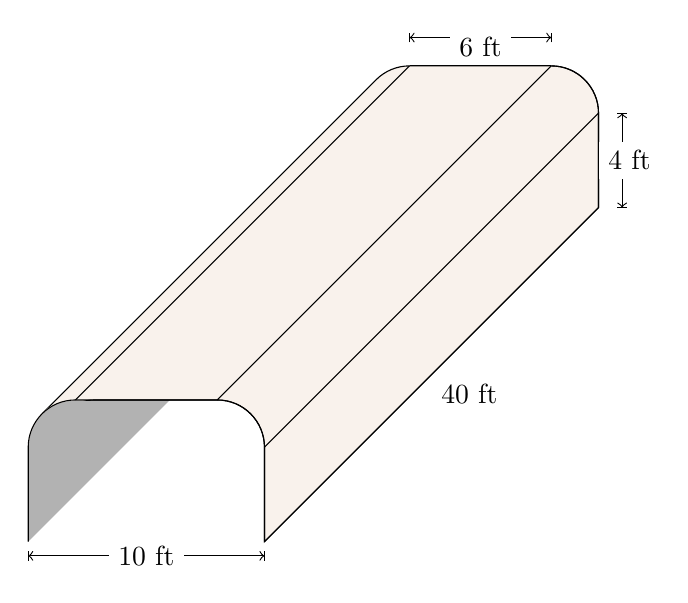
\begin{tikzpicture}[scale=0.6]
\fill[black!30](0,0)--(0,2)--++(45:10)--++(0,-2)--++(45:-10);
\fill[brown!10,draw=black](0.7071,2.7071)arc(135:90:1)--(4,3)arc(90:0:1)--(5,0) --++(45:10)--++(0,2)arc(0:90:1)--++(-3,0)arc(90:135:1)--++(45:-10);
\fill[black!30](0,2)arc(180:90:1)--++(0,-1)--++(-1,0);
\draw[brown!10](0,2)arc(180:90:1);
\draw[<->](5.5,0)++(45:10)--++(0,2);
\draw(5.4,0)++(45:10)--++(0.2,0)++(0,2)--++(-0.2,0);
\draw(1,3.5)++(45:10)--++(0,0.2)(4,3.5)++(45:10)--++(0,0.2);
\draw[<->](1,3.6)++(45:10)--++(3,0);
\draw(1,3)++(45:10)--++(1.5,0)node[anchor=south, rectangle, fill=white]{$6$ ft}--++(1.5,0);
\draw(0,-.2)--(0,-.4)(5,-.2)--(5,-.4);
\draw[<->](0,-.3)--(5,-.3);
\draw(2.5,-.3)node[rectangle, fill=white]{$10$ ft};
\draw(5,0)++(45:10)--++(0,1)node[anchor=west, rectangle, fill=white]{$4$ ft}--++(0,1)arc(0:90:1);
\draw(5,0)--++(45:5)node[anchor=north west]{$40$ ft}--++(45:5);
\draw(0,0)--(0,2)arc(180:90:1)--(4,3)arc(90:0:1)--(5,0);
\draw(5,2)--++(45:10)(4,3)--++(45:10)(1,3)--++(45:10);
\fill[black!30](0.98,2.98)rectangle(1.4,2.7);
\end{tikzpicture}\end{center}
Jeremy has a frame in the shape above he wishes to paint on both the inside and the outside.  The frame has $90$ degree partial cylinder sides connecting three rectangles.  The paint he wishes to use has a coverage of about $38$ square yards per gallon.  If Jeremy can only buy his desired paint in whole gallons, how many gallons should he buy?
\\\\


\ifsat
	\begin{enumerate}[label=\Alph*)]
	\end{enumerate}
\else
\fi

\ifacteven
	\begin{enumerate}[label=\textbf{\Alph*.},itemsep=\fill,align=left]
	\end{enumerate}
\else
\fi

\ifactodd
	\begin{enumerate}[label=\textbf{\Alph*.},itemsep=\fill,align=left]
	\end{enumerate}
\else
\fi

\ifgridin
$5 $
\else
\fi

